% Created by tikzDevice version 0.12.6 on 2026-10-29 12:50:56
% !TEX encoding = UTF-8 Unicode
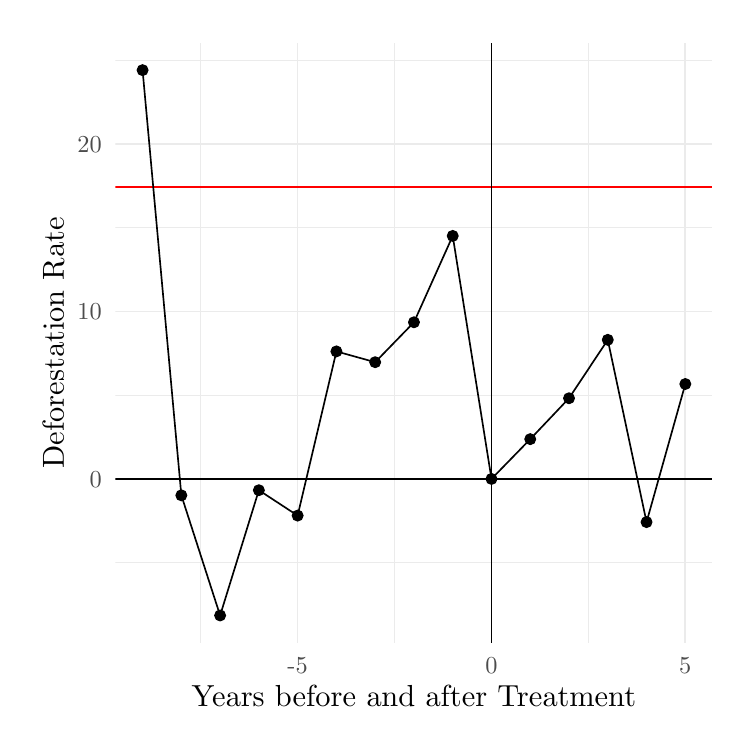
\begin{tikzpicture}[x=1pt,y=1pt]
\definecolor{fillColor}{RGB}{255,255,255}
\path[use as bounding box,fill=fillColor,fill opacity=0.00] (0,0) rectangle (252.94,252.94);
\begin{scope}
\path[clip] (  0.00,  0.00) rectangle (252.94,252.94);
\definecolor{fillColor}{RGB}{255,255,255}

\path[fill=fillColor] (  0.00,  0.00) rectangle (252.94,252.94);
\end{scope}
\begin{scope}
\path[clip] ( 31.71, 30.69) rectangle (247.44,247.45);
\definecolor{drawColor}{gray}{0.92}

\path[draw=drawColor,line width= 0.3pt,line join=round] ( 31.71, 59.62) --
	(247.44, 59.62);

\path[draw=drawColor,line width= 0.3pt,line join=round] ( 31.71,120.15) --
	(247.44,120.15);

\path[draw=drawColor,line width= 0.3pt,line join=round] ( 31.71,180.68) --
	(247.44,180.68);

\path[draw=drawColor,line width= 0.3pt,line join=round] ( 31.71,241.21) --
	(247.44,241.21);

\path[draw=drawColor,line width= 0.3pt,line join=round] ( 62.53, 30.69) --
	( 62.53,247.45);

\path[draw=drawColor,line width= 0.3pt,line join=round] (132.57, 30.69) --
	(132.57,247.45);

\path[draw=drawColor,line width= 0.3pt,line join=round] (202.62, 30.69) --
	(202.62,247.45);

\path[draw=drawColor,line width= 0.6pt,line join=round] ( 31.71, 89.88) --
	(247.44, 89.88);

\path[draw=drawColor,line width= 0.6pt,line join=round] ( 31.71,150.41) --
	(247.44,150.41);

\path[draw=drawColor,line width= 0.6pt,line join=round] ( 31.71,210.94) --
	(247.44,210.94);

\path[draw=drawColor,line width= 0.6pt,line join=round] ( 97.55, 30.69) --
	( 97.55,247.45);

\path[draw=drawColor,line width= 0.6pt,line join=round] (167.60, 30.69) --
	(167.60,247.45);

\path[draw=drawColor,line width= 0.6pt,line join=round] (237.64, 30.69) --
	(237.64,247.45);
\definecolor{drawColor}{RGB}{255,0,0}

\path[draw=drawColor,line width= 0.6pt,line join=round] ( 31.71,195.45) -- (247.44,195.45);
\definecolor{drawColor}{RGB}{0,0,0}

\path[draw=drawColor,line width= 0.6pt,line join=round] ( 41.52,237.59) --
	( 55.53, 83.95) --
	( 69.54, 40.54) --
	( 83.54, 85.80) --
	( 97.55, 76.63) --
	(111.56,135.96) --
	(125.57,132.06) --
	(139.58,146.48) --
	(153.59,177.69) --
	(167.60, 89.88) --
	(181.60,104.25) --
	(195.61,119.03) --
	(209.62,140.14) --
	(223.63, 74.28) --
	(237.64,124.18);
\definecolor{fillColor}{RGB}{0,0,0}

\path[draw=drawColor,line width= 0.4pt,line join=round,line cap=round,fill=fillColor] ( 41.52,237.59) circle (  1.96);

\path[draw=drawColor,line width= 0.4pt,line join=round,line cap=round,fill=fillColor] ( 55.53, 83.95) circle (  1.96);

\path[draw=drawColor,line width= 0.4pt,line join=round,line cap=round,fill=fillColor] ( 69.54, 40.54) circle (  1.96);

\path[draw=drawColor,line width= 0.4pt,line join=round,line cap=round,fill=fillColor] ( 83.54, 85.80) circle (  1.96);

\path[draw=drawColor,line width= 0.4pt,line join=round,line cap=round,fill=fillColor] ( 97.55, 76.63) circle (  1.96);

\path[draw=drawColor,line width= 0.4pt,line join=round,line cap=round,fill=fillColor] (111.56,135.96) circle (  1.96);

\path[draw=drawColor,line width= 0.4pt,line join=round,line cap=round,fill=fillColor] (125.57,132.06) circle (  1.96);

\path[draw=drawColor,line width= 0.4pt,line join=round,line cap=round,fill=fillColor] (139.58,146.48) circle (  1.96);

\path[draw=drawColor,line width= 0.4pt,line join=round,line cap=round,fill=fillColor] (153.59,177.69) circle (  1.96);

\path[draw=drawColor,line width= 0.4pt,line join=round,line cap=round,fill=fillColor] (181.60,104.25) circle (  1.96);

\path[draw=drawColor,line width= 0.4pt,line join=round,line cap=round,fill=fillColor] (195.61,119.03) circle (  1.96);

\path[draw=drawColor,line width= 0.4pt,line join=round,line cap=round,fill=fillColor] (209.62,140.14) circle (  1.96);

\path[draw=drawColor,line width= 0.4pt,line join=round,line cap=round,fill=fillColor] (223.63, 74.28) circle (  1.96);

\path[draw=drawColor,line width= 0.4pt,line join=round,line cap=round,fill=fillColor] (237.64,124.18) circle (  1.96);

\path[draw=drawColor,line width= 0.4pt,line join=round,line cap=round,fill=fillColor] (167.60, 89.88) circle (  1.96);
\definecolor{fillColor}{RGB}{51,51,51}

\path[fill=fillColor,fill opacity=0.20] ( 41.52,237.59) --
	( 55.53, 83.95) --
	( 69.54, 40.54) --
	( 83.54, 85.80) --
	( 97.55, 76.63) --
	(111.56,135.96) --
	(125.57,132.06) --
	(139.58,146.48) --
	(153.59,177.69) --
	(167.60, 89.88) --
	(181.60,104.25) --
	(195.61,119.03) --
	(209.62,140.14) --
	(223.63, 74.28) --
	(237.64,124.18) --
	(237.64,124.18) --
	(223.63, 74.28) --
	(209.62,140.14) --
	(195.61,119.03) --
	(181.60,104.25) --
	(167.60, 89.88) --
	(153.59,177.69) --
	(139.58,146.48) --
	(125.57,132.06) --
	(111.56,135.96) --
	( 97.55, 76.63) --
	( 83.54, 85.80) --
	( 69.54, 40.54) --
	( 55.53, 83.95) --
	( 41.52,237.59) --
	cycle;

\path[] ( 41.52,237.59) --
	( 55.53, 83.95) --
	( 69.54, 40.54) --
	( 83.54, 85.80) --
	( 97.55, 76.63) --
	(111.56,135.96) --
	(125.57,132.06) --
	(139.58,146.48) --
	(153.59,177.69) --
	(167.60, 89.88) --
	(181.60,104.25) --
	(195.61,119.03) --
	(209.62,140.14) --
	(223.63, 74.28) --
	(237.64,124.18);

\path[] (237.64,124.18) --
	(223.63, 74.28) --
	(209.62,140.14) --
	(195.61,119.03) --
	(181.60,104.25) --
	(167.60, 89.88) --
	(153.59,177.69) --
	(139.58,146.48) --
	(125.57,132.06) --
	(111.56,135.96) --
	( 97.55, 76.63) --
	( 83.54, 85.80) --
	( 69.54, 40.54) --
	( 55.53, 83.95) --
	( 41.52,237.59);

\path[draw=drawColor,line width= 0.6pt,line join=round] ( 31.71, 89.88) -- (247.44, 89.88);

\path[draw=drawColor,line width= 0.6pt,line join=round] (167.60, 30.69) -- (167.60,247.45);
\end{scope}
\begin{scope}
\path[clip] (  0.00,  0.00) rectangle (252.94,252.94);
\definecolor{drawColor}{gray}{0.30}

\node[text=drawColor,anchor=base east,inner sep=0pt, outer sep=0pt, scale=  0.88] at ( 26.76, 86.85) {0};

\node[text=drawColor,anchor=base east,inner sep=0pt, outer sep=0pt, scale=  0.88] at ( 26.76,147.38) {10};

\node[text=drawColor,anchor=base east,inner sep=0pt, outer sep=0pt, scale=  0.88] at ( 26.76,207.91) {20};
\end{scope}
\begin{scope}
\path[clip] (  0.00,  0.00) rectangle (252.94,252.94);
\definecolor{drawColor}{gray}{0.30}

\node[text=drawColor,anchor=base,inner sep=0pt, outer sep=0pt, scale=  0.88] at ( 97.55, 19.68) {-5};

\node[text=drawColor,anchor=base,inner sep=0pt, outer sep=0pt, scale=  0.88] at (167.60, 19.68) {0};

\node[text=drawColor,anchor=base,inner sep=0pt, outer sep=0pt, scale=  0.88] at (237.64, 19.68) {5};
\end{scope}
\begin{scope}
\path[clip] (  0.00,  0.00) rectangle (252.94,252.94);
\definecolor{drawColor}{RGB}{0,0,0}

\node[text=drawColor,anchor=base,inner sep=0pt, outer sep=0pt, scale=  1.10] at (139.58,  7.64) {Years before and after Treatment};
\end{scope}
\begin{scope}
\path[clip] (  0.00,  0.00) rectangle (252.94,252.94);
\definecolor{drawColor}{RGB}{0,0,0}

\node[text=drawColor,rotate= 90.00,anchor=base,inner sep=0pt, outer sep=0pt, scale=  1.10] at ( 13.08,139.07) {Deforestation Rate};
\end{scope}
\end{tikzpicture}
